\chapter{Convergence Tests for Series}

\section{Test for Divergence}
Recall from the previous chapter that if the terms of a series do not approach 
zero as $n$ approaches infinity, then the series is divergent. This is the 
Test for Divergence\index{Test for Divergence}, and there are two possible 
outcomes. For a series $\sum_{n = 1}^\infty a_n$:
$$\text{If } \lim_{n \to \infty} a_n \neq 0 \text{, then the series diverges}$$
$$\text{If } \lim_{n \to \infty} a_n = 0 \text{, then the test is inconclusive}$$

It is important to remember that the Test for Divergence cannot tell us 
conclusively that a series converges. Rather, it only identifies series that 
are divergent. 

\textbf{Example}: Apply the Test for Divergence to the series $\sum_{n=1}^
\infty \sqrt{n}$ and $\sum_{n=1}^\infty \frac{1}{n}$

\textbf{Solution}: $\lim_{n \to \infty} \sqrt{n} = \infty \neq 0$. Therefore, 
the series $\sum_{n=1}^\infty \sqrt{n}$ is divergent. 

$\lim_{n \to \infty} \frac{1}{n} = 0$. Therefore, the series $\sum_{n=1}^
\infty \frac{1}{n}$ may be divergent or convergent. This is the harmonic 
series, which we proved to be divergent in the previous chapter. This is a 
good example that demonstrates that just because $\lim_{n \to \infty} a_n = 
0$ does not mean the series is convergent. 

\section{The Integral Test}
We were able to determine the exact value of some infinite series because it 
was possible to write the $n^{th}$ partial sum, $s_n$, in terms of $n$. For 
example, we determined that the $n^{th}$ partial sum of $\sum_{i = 1}^n 
\frac{1}{2^i}$ is $s_n = 1 - \frac{1}{2^n}$. However, it is not always possible 
to do this. How can we estimate the value of an infinite series in cases where 
we can't explicitly write $s_n$ in terms of $n$? \index{Integral Test}

Consider the series $\sum_{i = 1}^\infty \frac{1}{i^2}$. The first few terms 
are:
$$\sum_{i = 1}^\infty \frac{1}{2^i} = \frac{1}{1^2} + \frac{1}{2^2} + 
\frac{1}{3^2} + \frac{1}{4^2} + \frac{1}{5^2} + \cdots$$

The series is decreasing, but is it convergent? Let's plot this series on an 
$xy$-plane (see figure \ref{fig:invsquare1}). 

\begin{figure}[htbp]
    \centering
    \begin{tikzpicture}
        \begin{axis}[xmin = -0.25, xmax = 6, axis lines = center, xlabel = $i$, 
        ymin = 0, ymax = 1.25, ytick = \empty, ylabel=$\frac{1}{2^i}$]
        \foreach \n in {1,...,5}{
        \addplot[red, mark=*]({\n}, {1/(\n)^2});
        }
        \end{axis}
    \end{tikzpicture}
    \caption{The first 5 terms of $\sum_{i = 1}^\infty \frac{1}{2^i}$}
    \label{fig:invsquare1}
\end{figure}

We can overlay the function $y = \frac{1}{2^x}$ (figure \ref{fig:invsquare2}). 
We can draw rectangles of width 1 and height $\frac{1}{x^2}$ (see figure 
\ref{fig:invsquare3}). The area of the first $n$ rectangles is equal to the 
$n^{th}$ partial sum. 

\begin{figure}[htbp]
    \centering
    \begin{tikzpicture}
        \begin{axis}[xmin = -0.25, xmax = 6, axis lines = center, 
        xlabel = $i$, ymin = 0, ymax = 1.25, ytick = \empty, ylabel=$\frac{1}{2^i}$]
        \foreach \n in {1,...,5}{
        \addplot[red, mark=*]({\n}, {1/(\n)^2});
        }
        \addplot[blue, domain = 0.7:6] {1/x^2};
        \end{axis}
    \end{tikzpicture}
    \caption{The first 5 terms of $\sum_{i = 1}^\infty \frac{1}{2^i}$ lie on 
    the curve $y = \frac{1}{x^2}$}
    \label{fig:invsquare2}
\end{figure}

\begin{figure}[htbp]
    \centering
    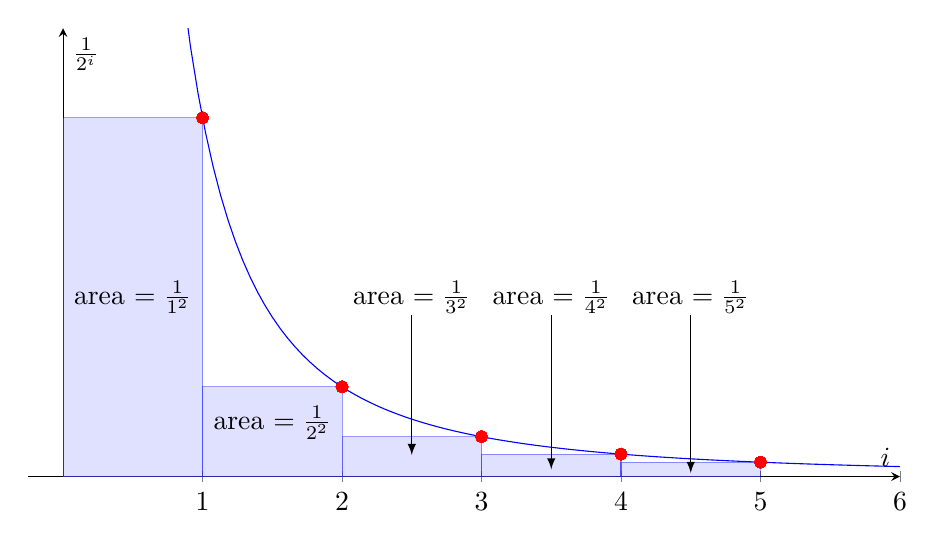
\begin{tikzpicture}
        \begin{axis}[xmin = -0.25, xmax = 6, axis lines = center, xlabel = $i$, 
        ymin = 0, ymax = 1.25, ytick = \empty, width = 1.5*\axisdefaultwidth, 
        height = \axisdefaultheight, ylabel=$\frac{1}{2^i}$]
        \foreach \n in {1,...,5}{
        \addplot[red, mark=*]({\n}, {1/(\n)^2});
        }
        \addplot[blue, domain = 0.7:6, samples=100] {1/x^2};
        \filldraw[fill=blue!30, draw = blue, opacity = 0.4] 
        (0, 0) rectangle (1,  1);
        \filldraw[fill=blue!30, draw = blue, opacity = 0.4] 
        (1, 0) rectangle (2, 0.25);
        \filldraw[fill=blue!30, draw = blue, opacity = 0.4] 
        (2, 0) rectangle (3,  1/9);
        \filldraw[fill=blue!30, draw = blue, opacity = 0.4] 
        (3, 0) rectangle (4,  1/16);
        \filldraw[fill=blue!30, draw = blue, opacity = 0.4] 
        (4, 0) rectangle (5,  1/25);
        \node[] at (0.5, 0.5) {area $=\frac{1}{1^2}$};
        \node[] at (1.5, 0.15) {area $=\frac{1}{2^2}$};
        \node[] at (2.5, 0.5) {area $=\frac{1}{3^2}$};
        \node[] at (3.5, 0.5) {area $=\frac{1}{4^2}$};
        \node[] at (4.5, 0.5) {area $=\frac{1}{5^2}$};
        \draw[-latex](2.5, 0.45) -- (2.5, 0.06);
        \draw[-latex](3.5, 0.45) -- (3.5, 0.02);
        \draw[-latex](4.5, 0.45) -- (4.5, 0.01);
        \end{axis}
    \end{tikzpicture}
    \caption{The partial sum $\sum_{i=1}^{n=5} \frac{1}{2^i}$ is equal to the 
    area of the rectangles}
    \label{fig:invsquare3}
\end{figure}

This should remind you of a Riemann sum. Since the total area of the rectangles 
is less than the area under the curve, we can state:
$$\sum_{i = 1}^\infty \frac{1}{2^i} < \int_0^\infty \frac{1}{x^2}\,dx$$

We can exclude the first rectangle and also state that: 
$$\sum_{i = 1}^\infty \frac{1}{2^i}< 1 + \int_1^\infty \frac{1}{x^2}\,dx$$

We can evaluate this integral:
$$\int_1^\infty \frac{1}{x^2}\,dx = \lim_{t \to \infty} \left[ \int_1^t 
\frac{1}{x^2}\,dx \right]$$
$$ = \lim_{t \to \infty} \frac{-1}{x}|_{x=1}^t = \lim_{t \to \infty} \left( 
\frac{-1}{t} \right) - \frac{-1}{1} = 0 - (-1) = 1$$

Therefore:
$$\sum_{i = 1}^\infty \frac{1}{2^i}< 1 + 1 = 2$$

This means the series $\sum_{i = 1}^\infty \frac{1}{2^i}$ is bounded above. 
Since the series is also monotonic (each term is positive, so the value of the 
sum increases as $n$ increases), we can state that the sum is convergent! 

Let's look at a divergent example: $\sum_{i = 1}^\infty \frac{1}{\sqrt{x}}$. 
Again, we will make a visual, but this time we will draw rectangles that lie 
above the curve $y = \frac{1}{\sqrt{x}}$ (see figure \ref{fig:invroot}). In 
this case, $\sum_{i = 1}^\infty \frac{1}{\sqrt{x}}> \int_1^\infty 
\frac{1}{\sqrt{x}}\,dx$. Let's evaluate the integral:
$$\int_1^\infty \frac{1}{\sqrt{x}}\,dx = \lim_{t \to \infty} \left[ \int_1^t 
\frac{1}{\sqrt{x}}\,dx \right] $$
$$= \lim_{t \to \infty} \left[ 2 \sqrt{x} \right]_{x=1}^t= \lim_{t \to \infty} 
\left( 2\sqrt{t} \right) - 2\sqrt{1} = \infty - 2 \rightarrow \text{divergent}$$

Since the integral diverges to infinity and the series is greater than the 
integral, the series must also diverge to infinity. This is another case where 
a monotonic decreasing series is not convergent!

\begin{figure}[htbp]
    \centering
    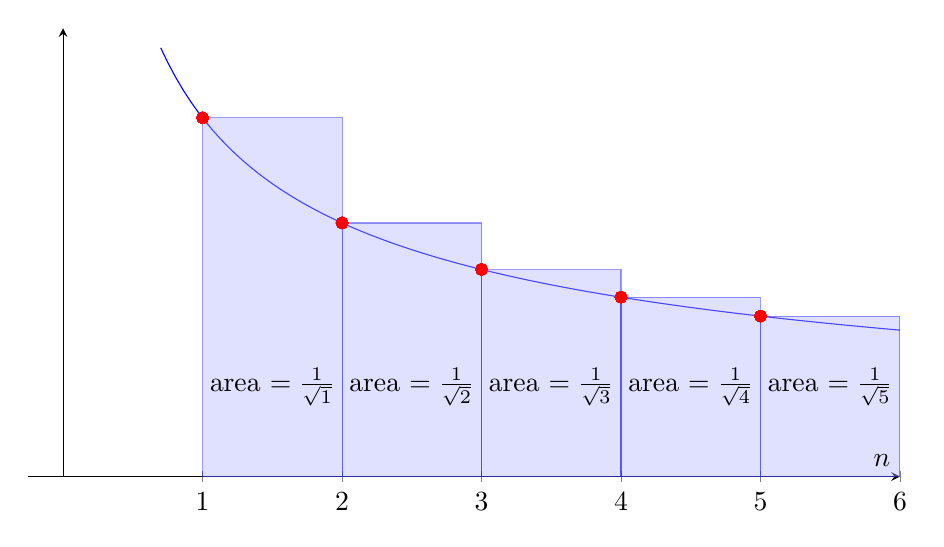
\begin{tikzpicture}
        \begin{axis}[xmin = -0.25, xmax = 6, axis lines = center, xlabel = $n$, 
        ymin = 0, ymax = 1.25, ytick = \empty, width = 1.5*\axisdefaultwidth, 
        height = \axisdefaultheight]
        \foreach \n in {1,...,5}{
        \addplot[red, mark=*]({\n}, {1/sqrt(\n)});
        }
        \addplot[blue, domain = 0.7:6, samples=100] {1/sqrt(x)};
        \filldraw[fill=blue!30, draw = blue, opacity = 0.4] 
        (1, 0) rectangle (2,  1);
        \filldraw[fill=blue!30, draw = blue, opacity = 0.4] 
        (2, 0) rectangle (3, 0.707);
        \filldraw[fill=blue!30, draw = blue, opacity = 0.4] 
        (3, 0) rectangle (4,  0.577);
        \filldraw[fill=blue!30, draw = blue, opacity = 0.4] 
        (4, 0) rectangle (5,  0.5);
        \filldraw[fill=blue!30, draw = blue, opacity = 0.4] 
        (5, 0) rectangle (6, 0.4472);
        \node[] at (1.5, 0.25) {area $=\frac{1}{\sqrt{1}}$};
        \node[] at (2.5, 0.25) {area $=\frac{1}{\sqrt{2}}$};
        \node[] at (3.5, 0.25) {area $=\frac{1}{\sqrt{3}}$};
        \node[] at (4.5, 0.25) {area $=\frac{1}{\sqrt{4}}$};
        \node[] at (5.5, 0.25) {area $=\frac{1}{\sqrt{5}}$};
        \end{axis}
    \end{tikzpicture}
    \caption{$\sum_{i = 1}^\infty \frac{1}{\sqrt{x}}> \int_1^\infty 
    \frac{1}{\sqrt{x}}\,dx$}
    \label{fig:invroot}
\end{figure}

This leads us to the \textbf{Integral Test}. If $f$ is a continuous, positive, 
decreasing function on the interval $x \in [1, \infty)$ and $a_n = f(n)$, then 
the series $\sum_{n=1}^\infty a_n$ converges if and only if $\int_1^\infty 
f(x)\,dx$ is convergent. Subsequently, if $\int_1^\infty f(x)\,dx$ is 
divergent, then the series is also divergent.

\textbf{Example}: Is the series $\sum_{i = 1}^\infty \frac{1}{n^2 + 1}$ 
convergent or divergent?

\textbf{Solution}: To apply the integral test, we define $f(x) = 
\frac{1}{x^2 + 1}$, which is a positive, decreasing function on the interval 
$x \in [1, \infty)$. 
$$\int_1^\infty \frac{1}{x^2 + 1}\,dx = \lim_{t \to \infty} \int_{1}^t 
\frac{1}{x^2 + 1}\,dx$$
$$= \lim_{t \to \infty} \left[ \arctan{x} \right]_{x = 1}^t = \lim_{t \to \infty} 
\left( \arctan{t} \right) - \arctan{1} = \frac{\pi}{2} - \frac{\pi}{4} = 
\frac{\pi}{4}$$

Because the integral $\int_1^\infty \frac{1}{x^2 + 1}\,dx$ converges, so does 
the series $\sum_{n = 1}^\infty \frac{1}{n^2 + 1}$. 

\begin{Exercise}[label = series1]
Use the integral test to determine if the following series are convergent or 
divergent. 
\begin{enumerate}
\item $\sum_{n = 1}^\infty 2n^{-3}$
\item $\sum_{n = 1}^\infty \frac{5}{3n-1}$
\item $\sum_{n = 1}^\infty \frac{n}{3n^2 + 1}$
\end{enumerate}
\vspace{40mm}
\end{Exercise}

\begin{Answer}[ref= series1]
\begin{enumerate}
\item The function $2x^{-3}$ is positive and decreasing for $x \in [1, \infty)$. 
$\int_1^\infty 2x^{-3}\,dx = \lim_{t \to \infty} \int_1^t 2x^{-3}\,dx = \lim_{t 
\to \infty} \left[-x^{-2} \right]_{x = 1}^t = \lim_{t \to \infty} ( -t^{-2}) - 
-(1)^{-2} = 0 + 1 = 1$. Since the integral $\int_1^\infty 2x^{-3}\,dx$ converges, 
the series $\sum_{n = 1}^\infty 2n^{-3}$ is also convergent.
\item The function $\frac{5}{3x+1}$ is positive and decreasing for $x \in [1, 
\infty)$. $\int_1^\infty \frac{5}{3x-1}\,dx = \lim_{t \to \infty} \int_1^t 
\frac{5}{3x-1}\,dx$ Using u-substitution to evaluate the integral, we set $u = 
3x-1$ and find that $du = 3dx \rightarrow dx = \frac{du}{3}$. Substituting, 
$\int_1^t \frac{5}{3x-1}\,dx = \int_{x=1}^{x=t} \frac{5}{3}\frac{1}{u}\,du$. 
Evaluating the integral, $\int_{x=1}^{x=t} \frac{5}{3}\frac{1}{u}\,du = 
\frac{5}{3}\ln{u}|_{x = 1}^{x =t} = \frac{5}{3}\ln{3x+1}|_{1}^t$. Substituting 
this back into the limit, $\int_1^\infty \frac{5}{3x-1}\,dx = \lim_{t \to 
\infty} \frac{5}{3}\ln{3x+1}|_{1}^t = \lim_{t \to \infty} [ \frac{5}{3} 
\ln{3t+1} ] - \frac{5}{3}\ln{4} = \infty - \frac{5}{3}\ln{4} = \infty$. 
Therefore, the integral $\int_1^\infty \frac{5}{3x-1}\,dx$ is divergent and so 
is the series $\sum_{n = 1}^\infty \frac{5}{3n-1}$.
\item The function $\frac{x}{3x^2 + 1}$ is positive and decreasing for $x\in 
[1,\infty)$. $\int_1^\infty \frac{x}{3x^2 + 1}\,dx = \lim_{t \to \infty} 
\int_1^t \frac{x}{3x^2 + 1}\,dx$. Applying the substitution $u = 3x^2 + 1$ 
and $\frac{du}{6} = x\text{ }dx$, we see that $\lim_{t \to \infty} \int_1^t 
\frac{x}{3x^2 + 1}\,dx = \lim_{t \to \infty} \int_{x=1}^{x=t} \frac{1}{6u}\,du 
= \lim_{t \to \infty} \frac{1}{6}\ln{u}|_{x = 1}^{x = t} = \lim_{t \to \infty} 
\frac{1}{6}\ln{3x^2 + 1}|_{1}^{t} = \lim_{t \to \infty} \left[ \frac{1}{6}
\ln{3t^2 + 1} \right] - \frac{1}{6}\ln{4} = \infty$. Therefore, the integral 
$\int_1^\infty \frac{x}{3x^2 + 1}\,dx$ is divergent, and so is the series 
$\sum_{n = 1}^\infty \frac{n}{3n^2 + 1}$. 
\end{enumerate}
\end{Answer}

\begin{Exercise}[label = pseries]
Apply the Integral Test to show that $p$-series $\sum_{n=1}^\infty \frac{1}{
n^p}$ are convergent only when $p > 1$ (hint: consider the cases $p \leq 0$, 
$0 < p < 1$, $p=1$ and $p > 1$).
\vspace{50mm}
\end{Exercise}

\begin{Answer}[ref = pseries]
\begin{enumerate}
\item If $p \leq 0$, then $\lim_{n \to \infty} \frac{1}{n^p} \neq 0$, and the 
series fails the Test for Divergence. Therefore, a $p$-series is divergent if 
$p \leq 0$. 
\item If $p > 0$, then $f(x) = \frac{1}{x^p}$ is continuous, positive, and 
decreasing on the interval $x \in [1, \infty)$, and we can apply the integral 
test. So, we want to know, when is $\int_1^\infty \frac{1}{x^p}\,dx$ convergent? 
When $p=1$, $\int_1^\infty \frac{1}{x^p}\,dx = \ln{x}|_{x=1}^{x=\infty} = \lim_
{t \to \infty} \ln{t} - \ln{1} = \infty$ and the integral and $p$-series are 
both divergent.
\item What about when $0 < p < 1$? In this case, the integral $\int_1^\infty \frac{1}{
x^p}\,dx = \lim_{t \to \infty} \int_1^t x^{-p}\,dx = \lim_{t \to \infty} 
\frac{1}{1-p}x^{1-p}|_{x=1}^{x=t} = \lim_{t \to \infty} \frac{1}{1-p}\frac{1}{
x^{p-1}} = \left( \frac{1}{1-p} \right) \left[\lim_{t \to \infty} \left( \frac{
1}{t^{p-1}} \right) - 1 \right]$. When $0 < p < 1$, then $1 - p > 0$ is 
positive and $\lim_{t \to \infty} \frac{1}{t^{p-1}} = \lim_{t \to \infty} t^{1-
p} = \infty$ and the integral diverges. Therefore, $p$-series are divergent for 
$0 < p < 1$.
\item When $p > 1$, then $\int_1^\infty \frac{1}{x^p}\,dx = \left( \frac{1}{1-
p} \right) \left[\lim_{t \to \infty} \left( \frac{1}{t^{p-1}} \right) - 1 
\right]$. When $p > 1$, $p - 1 > 0$ and $\lim_{t \to \infty} \frac{1}{t^{p-1}} 
= 0$. Therefore, $\int_{1}^\infty \frac{1}{x^p}\,dx$ converges to $\frac{1}{p 
- 1}$ when $p > 1$, and therefore the $p$-series is convergent when $p > 1$. 
\end{enumerate}
\end{Answer}

\subsection{Using Integrals to Estimate the Value of a Series}
Recall that $\sum_{i=1}^\infty a_i = a_1 + a_2 + a_3 + \cdots = s$ and that 
the $n^{th}$ partial sum, often represented as $s_n$, is $s_n = a_1 + a_2 + 
\cdots + a_{n-1} + a_n$. We can then define the $n^{th}$ remainder $R_n = s - 
s_n$.\index{remainder estimate for series} Expanding $s$ and $s_n$, we see that:
$$R_n = \left[ a_1 + a_2 + \cdots + a_{n-1} + a_n + a_{n+1} + \cdots \right] - 
\left[ a_1 + a_2 + \cdots + a_{n-1} + a_{n} \right]$$
$$R_n = [a_1 - a_1] + [a_2 - a_2] + \cdots + [a_{n-1} - a_{n-1}] + [a_n - a_n] 
+ a_{n-1} + a_{n-2} + \cdots$$
$$R_n = a_{n+1} + a_{n+2} + a_{n+3} + \cdots$$

Just like the integral test, suppose there is some continuous, positive, 
decreasing function, such that $a_n = f(n)$. We can then represent $R_n$ as the 
right Riemann sum with width $\Delta x = 1$ from $x = n$ to $\infty$. Since 
the rectangles are below the curve (see figure \ref{fig:remainderceiling}), we 
can state that $R_n \leq \int_n^\infty f(x)\,dx$.

\begin{figure}[htbp]
    \centering
    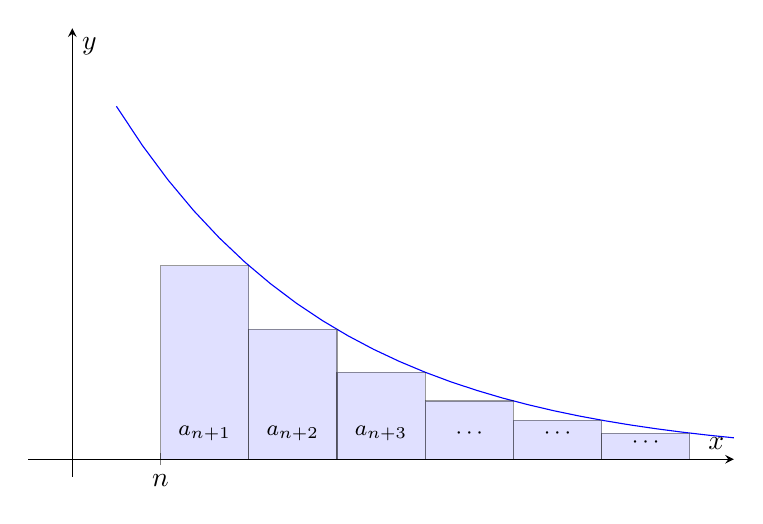
\begin{tikzpicture}
        \begin{axis}[xmin = -0.1, xmax = 1.5, axis lines = center, 
        xlabel = $x$, ymin = -0.2, ymax = 5, ytick = \empty, 
        width = 1.25*\axisdefaultwidth, height = \axisdefaultheight, 
        xtick={0.2}, xticklabels={$n$}, ylabel={$y$}]
        \addplot[blue, domain = 0.1:1.5]{5*e^(-2*x)};
        \filldraw[fill=blue!30, draw=black, opacity = 0.4] 
        (0.2, 0) rectangle (0.4, {5*e^(-2*0.4)});
        \filldraw[fill=blue!30, draw=black, opacity = 0.4] 
        (0.4, 0) rectangle (0.6, {5*e^(-2*0.6)});
        \filldraw[fill=blue!30, draw=black, opacity = 0.4] 
        (0.6, 0) rectangle (0.8, {5*e^(-2*0.8)});
        \filldraw[fill=blue!30, draw=black, opacity = 0.4] 
        (0.8, 0) rectangle (1, {5*e^(-2*1)});
        \filldraw[fill=blue!30, draw=black, opacity = 0.4] 
        (1, 0) rectangle (1.2, {5*e^(-2*1.2)});
        \filldraw[fill=blue!30, draw=black, opacity = 0.4] 
        (1.2, 0) rectangle (1.4, {5*e^(-2*1.4)});
        \node[font=\footnotesize] at (0.3, 0.3) {$a_{n+1}$};
        \node[font=\footnotesize] at (0.5, 0.3) {$a_{n+2}$};
        \node[font=\footnotesize] at (0.7, 0.3) {$a_{n+3}$};
        \node[font=\footnotesize] at (0.9, 0.3) {$\cdots$};
        \node[font=\footnotesize] at (1.1, 0.3) {$\cdots$};
        \node[font=\footnotesize] at (1.3, 0.2) {$\cdots$};
        \end{axis}
    \end{tikzpicture}
    \caption{$R_n \leq \int_n^\infty f(x)\,dx$ }
    \label{fig:remainderceiling}
\end{figure}

Similarly, we can represent $R_n$ as the left Riemann sum with width $\Delta x 
= 1$ from $x= n + 1$ to $\infty$. This time, the rectangles are above the curve 
(see figure \ref{fig:remainderfloor}), and we can state that $R_n \geq \int_
{n+1}^\infty f(x)\,dx$. Putting this all together, we have an estimate for the 
remainder, $R_n$, from the integral test:

Suppose there is a function such that $f(k) = a_k$, where $f$ is a continuous, 
positive, decreasing function for $x \geq n$ and $\sum a_n$ is convergent. 
Then, $\int_{n+1}^\infty f(x)\,dx \leq R_n \leq \int_n^\infty f(x)\,dx$, where 
$R_n$ is $s - s_n$. 

\begin{figure}[htbp]
    \centering
    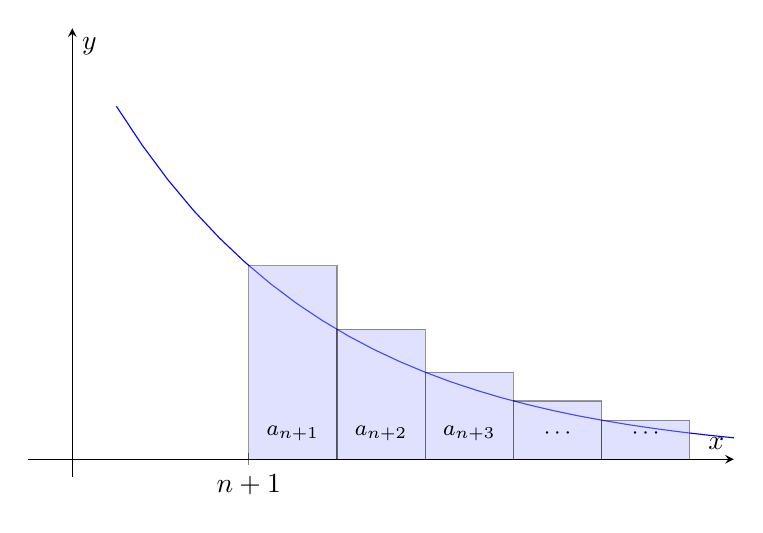
\begin{tikzpicture}
        \begin{axis}[xmin = -0.1, xmax = 1.5, axis lines = center, 
        xlabel = $x$, ymin = -0.2, ymax = 5, ytick = \empty, 
        width = 1.25*\axisdefaultwidth, height = \axisdefaultheight, 
        xtick={0.4}, xticklabels={$n+1$}, ylabel={$y$}]
        \addplot[blue, domain = 0.1:1.5]{5*e^(-2*x)};
        \filldraw[fill=blue!30, draw=black, opacity = 0.4] 
        (0.4, 0) rectangle (0.6, {5*e^(-2*0.4)});
        \filldraw[fill=blue!30, draw=black, opacity = 0.4] 
        (0.6, 0) rectangle (0.8, {5*e^(-2*0.6)});
        \filldraw[fill=blue!30, draw=black, opacity = 0.4] 
        (0.8, 0) rectangle (1, {5*e^(-2*0.8)});
        \filldraw[fill=blue!30, draw=black, opacity = 0.4] 
        (1, 0) rectangle (1.2, {5*e^(-2*1)});
        \filldraw[fill=blue!30, draw=black, opacity = 0.4] 
        (1.2, 0) rectangle (1.4, {5*e^(-2*1.2)});
        \node[font=\footnotesize] at (0.5, 0.3) {$a_{n+1}$};
        \node[font=\footnotesize] at (0.7, 0.3) {$a_{n+2}$};
        \node[font=\footnotesize] at (0.9, 0.3) {$a_{n+3}$};
        \node[font=\footnotesize] at (1.1, 0.3) {$\cdots$};
        \node[font=\footnotesize] at (1.3, 0.3) {$\cdots$};
        \end{axis}
    \end{tikzpicture}
    \caption{$R_n \geq \int_{n+1}^\infty f(x)\,dx$ }
    \label{fig:remainderfloor}
\end{figure}

\textbf{Example}: Approximate the sum of the series $\sum_{n=1}^\infty 
\frac{3}{n^3}$ by finding the $10^{th}$ partial sum. Estimate the error of 
this approximation. 

\textbf{Solution}: Using a calculator, you can find the $10^{th}$ partial sum: 
$$\sum_{n=1}^{10} \frac{3}{n^3} = \frac{3}{1^3} + \frac{3}{2^3} + 
\frac{3}{3^3} + \cdots + \frac{3}{10^3} \approx 3.593 = s_{10}$$

Recall that the remainder, $R_{10}$, is the difference between the actual sum, 
$s$, and the partial sum, $s_{10}$. Using the integral test to estimate the 
remainder, we can state that: $$R_{10} \leq \int_{10}^\infty \frac{3}{x^3}\,dx 
= \frac{3}{2(10)^2} = \frac{3}{200} = 0.015$$ Therefore, the size of the error 
is at most 0.015. 

\textbf{Example}: How many terms are required for the error to be less than 
0.0001 for the sum presented above?

\textbf{Solution}: We are looking for an $n$ such that $R_n \leq 0.0001$. 
Recalling that $R_n \leq \int_{n}^\infty \frac{3}{x^3}\,dx$, we need to find 
an $n$ such that $\int_{n}^\infty \frac{3}{x^3}\,dx \leq 0.0001$. 

$$\int_n^\infty \frac{3}{x^3}\,dx \leq 0.0001$$
$$\frac{-1}{6x^2}|_{x=n}^\infty \leq 0.0001$$
$$\lim_{x \to \infty} \frac{-1}{6x^2} - \frac{-1}{6n^2} \leq 0.0001$$
$$0 + \frac{1}{6n^2} = \frac{1}{6n^2} \leq 0.0001$$
$$1 \leq 0.0006n^2$$
$$1667 \leq n^2$$
$$40.8 \leq n \rightarrow n = 41$$
Therefore, $s - s_{41} \leq 0.0001$ and the partial sum $\Sigma_{n=1}^{41} 
\frac{3}{n^3}$ is less than 0.0001 from the value of the infinite sum $\sum_
{n=1}^\infty \frac{3}{n^3}$.

\begin{Exercise}[label=remainder1]
\begin{enumerate}
\item Find the partial sum $s_{10}$ of the series $\sum_{n=1}^\infty 
\frac{1}{n^4}$. 
\item Estimate the error from using $s_{10}$ as an approximation of the series.
\item Use $s_n + \int_{n+1}^\infty \frac{1}{x^4}\,dx \leq s \leq s_n + \int_n^
\infty \frac{1}{x^4}\,dx$ to give an improved estimate of the sum.
\item The actual value of $\sum_{n=1}^\infty \frac{1}{n^4}$ is 
$\frac{\pi^4}{90}$. Compare your estimate with the actual value.
\item Find a value of $n$ such that $s_n$ is within 0.00001 of the sum. 
\end{enumerate}
\vspace{50mm}
\end{Exercise}

\begin{Answer}[ref=remainder1]
\begin{enumerate}
\item $s_{10} = \frac{1}{1^4} + \frac{1}{2^4} + \cdots + \frac{1}{10^4} \approx 
1.082037$. 
\item $R_{10} \leq \int_{10}^\infty \frac{1}{x^4}\,dx = \frac{-1}{3x^3}|_
{x=10}^\infty = \lim_{x \to \infty} \frac{-1}{3x^3} - \frac{-1}{3 \cdot 10^3} 
= \frac{1}{3000} = 0.000333$. Therefore, the error is less than 0.000333. 
\item Given $s_{10} \approx 1.082037$, we can say that $1.082037 + \int_{n+1}^
\infty \frac{1}{x^4}\,dx \leq s \leq 1.082037 + \int_{n}^{\infty} \frac{1}{x^4}
\,dx$. Using a calculator to evaluate each integral, we see that: $1.082037 + 
0.000250 \leq s \leq 1.082037 + 0.000333$ and therefore the sum is between 
1.082287 and 1.082370. 
\item Writing the actual value as a decimal, $\frac{\pi^4}{90} \approx 
1.082323$, which is in the estimate window from the previous part. 
\item We are looking for an $n$ such that $\int_n^\infty \frac{1}{x^4}\,dx 
\leq 0.00001$. $\lim_{x \to \infty} \frac{-1}{3x^3} - \frac{-1}{3n^3} = 
\frac{1}{3n^3} \leq 0.00001$. $100,000 \leq 3n^3$. $33,333.33 \leq n^3$. 
$32.183 \leq n$. Since $n$ must be an integer, $n=33$ gives $R_n \leq 0.00001$. 
\end{enumerate}
\end{Answer}

\section{Comparison Tests}
\index{comparison tests for series} In comparison tests, we compare a series 
to a known convergent or divergent series. Take the series $\sum_{n=1}^\infty 
\frac{1}{3^n + 3}$. This is similar to $\sum_{n=1}^\infty \frac{1}{3^n}$, 
which is a geometric series that converges to $\frac{1}{2}$. Notice that:
$$\frac{1}{3^n + 3} < \frac{1}{3^n}$$
Which implies that 
$$\sum_{n=1}^\infty \frac{1}{3^n + 3} < \Sigma_{n=1}^\infty \frac{1}{3^n}$$

Since $\sum_{n=1}^\infty \frac{1}{3^n}$ is convergent, it follows that 
$\sum_{n=1}^\infty \frac{1}{3^n + 3}$ is also convergent (see figure 
\ref{fig:compare1}). As you can see, since  $\sum_{n=1}^\infty \frac{1}{3^n}$ 
approaches $\frac{1}{2}$, $\sum_{n=1}^\infty \frac{1}{3^n + 3}$ must be $\leq 
\frac{1}{2}$ and therefore convergent. 

\begin{figure}
    \centering
    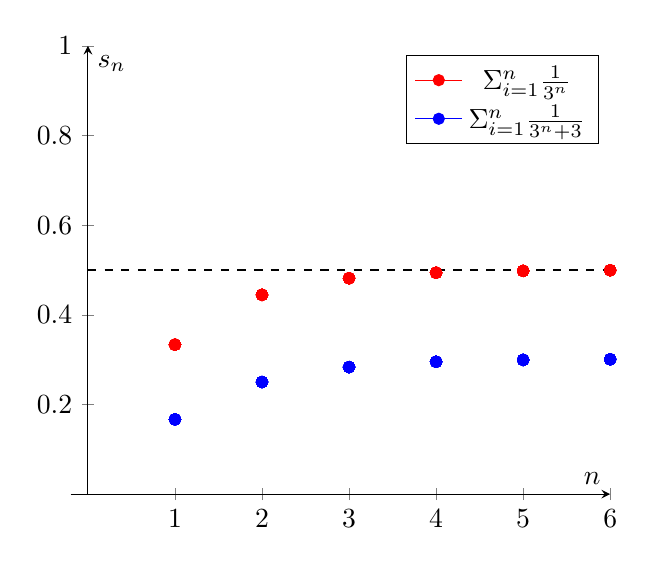
\begin{tikzpicture}
        \begin{axis}[xmin=-0.2, xmax = 6, ymin = 0, ymax=1, 
        axis lines = center, xlabel=$n$, ylabel = $s_n$]
        \addplot[red, mark=*](1, 1/3);
        \addlegendentry{$\Sigma_{i=1}^n \frac{1}{3^n}$};
        \addplot[blue, mark=*](1, 1/6);
        \addlegendentry{$\Sigma_{i=1}^n \frac{1}{3^n+3}$};
        \addplot[red, mark=*](2, 4/9);
        \addplot[red, mark=*](3, 13/27);
        \addplot[red, mark=*](4, 40/81);
        \addplot[red, mark=*](5, 121/243);
        \addplot[red, mark=*](6, 364/729);
        \addplot[blue, mark=*](2, 1/4);
        \addplot[blue, mark=*](3, 17/60);
        \addplot[blue, mark=*](4, 31/105);
        \addplot[blue, mark=*](5, 859/2870);
        \addplot[blue, mark=*](6, 315829/1050420);
        \addplot[black, dashed, domain = 0:6]{0.5};
        \end{axis}
    \end{tikzpicture}
    \caption{$\sum_{i=1}^n \frac{1}{3^n + 3} < \Sigma_{i = 1}^n 
    \frac{1}{3^n}$ for all $n$}
    \label{fig:compare1}
\end{figure}
\subsection{The Direct Comparison Test}
\index{Direct Comparison Test}For the \textbf{Direct Comparison Test}, we 
compare the terms $a_n$ to $b_n$ directly. Take $\sum a_n$ and $\sum b_n$ to 
be series with positive terms. Then, 
\begin{enumerate}
\item If $a_n \leq b_n$ and $\sum b_n$ is convergent, then $\sum a_n$ is 
also convergent.
\item If $a_n \geq b_n$ and $\sum b_n$ is divergent, then $\sum a_n$ is 
also divergent.
\end{enumerate}

We already discussed above why the first part is true. The second part follows 
a similar argument: If $a_n$ is greater than $b_n$, then you can imagine that 
as $\sum b_n$ grows and diverges, it is pushing upwards on $\sum a_n$, 
meaning that $\sum a_n$ must also diverge. Consider the series $\sum_{n=1}^
\infty \frac{2\ln{n}}{n}$. For $n \geq 2$, $2\ln{n} > 1$, and therefore if 
$\sum_{n=1}^\infty \frac{1}{n}$ diverges, then $\sum_{n=1}^\infty \frac{2
\ln{n}}{n}$ must also diverge. We recognize the harmonic series $\sum_{n=1}^
\infty \frac{1}{n}$ is divergent. Therefore, $\sum_{n=1}^\infty 
\frac{2\ln{n}}{n}$ is also divergent (see figure \ref{fig:compare2}).

\begin{figure}
    \centering
    \begin{tikzpicture}
        \begin{axis}[xmin=-0.2, xmax = 8, ymin = 0, axis lines = center, 
        xlabel=$n$, ylabel = $s_n$, legend style={at={(0.45,1)}}]
        \addplot[red, mark=*, only marks] coordinates {(1, 1) (2, 3/2) 
        (3, 11/6) (4, 25/12) (5, 137/60) (6, 49/20) (7, 363/140) (8, 761/280)};
        \addlegendentry{$\Sigma_{i=1}^n \frac{1}{n}$};
        \addplot[blue, mark=*, only marks] coordinates {(1, 0) (2, 0.693) 
        (3, 1.426) (4, 2.119) (5, 2.762) (6, 3.360) (7, 3.916) (8, 4.436)};
        \addlegendentry{$\sum_{i=1}^n \frac{2\ln{n}}{n}$};
        \end{axis}
    \end{tikzpicture}
    \caption{$\sum_{i=1}^n \frac{2\ln{n}}{n} > \sum_{i=1}^n \frac{1}{n}$ 
    for $n \geq 4$}
    \label{fig:compare2}
\end{figure}

\subsection{The Limit Comparison Test}
\index{Limit Comparison Test}Consider the series $\sum_{n=1}^\infty 
\frac{1}{2^n - 1}$. We may want to compare this to the convergent series $\sum_
{n=1}^\infty \frac{1}{2^n}$. The direct comparison test isn't helpful here, 
since $\frac{1}{2^n - 1} > \frac{1}{2^n}$, so $\sum_{n=1}^\infty \frac{1}{2^n}$ 
doesn't put a cap on $\sum_{n=1}^\infty \frac{1}{2^n - 1}$ like our earlier 
example (see figure \ref{fig:compare1}). In a case such as this, we can use 
the \textbf{Limit Comparison Test}, which states that:\\
If $\sum a_n$ and $\sum b_n$ are series with positive terms and $\lim_{n \to 
\infty} \frac{a_n}{b_n} = c > 0$, then either both series converge or both 
series diverge.

Let's apply this to the series $\sum_{n=1}^\infty \frac{1}{2^n - 1}$. We know 
that $\sum_{n=1}^\infty \frac{1}{2^n}$ converges, since it is a geometric 
series with $r < 1$. 
$$\lim_{n \to \infty} \frac{\frac{1}{2^n - 1}}{\frac{1}{2^n}} = \lim_{n \to 
\infty} \frac{1}{2^n - 1} \cdot \frac{2^n}{1}$$
$$= \lim_{n \to \infty} \frac{2^n}{2^n - 1} = \lim_{n \to \infty} \frac{1}{1 - 
1/2^n} = \frac{1}{1-0} = 1 > 0$$

Therefore, by the Limit Comparison Test, $\sum_{n=1}^\infty \frac{1}{2^n - 1}$ 
converges.

In general, comparison tests are most useful for series resembling geometric 
or $p$-series. When choosing a $p$-series to compare the unknown series to, 
choose $p$ such that the order of your $p$ series is the same as the order of 
the unknown series.

\textbf{Example}: What $p$-series should one compare the series $\sum_{n=1}^
\infty \frac{\sqrt{n^3 + 1}}{3n^3 + 4n^2 + 2}$ to?

\textbf{Solution}: We can determine the order of $\frac{\sqrt{n^3 + 1}}{3n^3 
+ 4n^2 + 2}$ by looking at the highest-order terms in the numerator and 
denominator:
$$\frac{\sqrt{n^3}}{n^3} = \frac{n^{3/2}}{n^3} = \frac{1}{n^{3/2}}$$
So, we should compare $\sum_{n=1}^\infty \frac{\sqrt{n^3 + 1}}{3n^3 + 4n^2 + 2}$ 
to the convergent $p$-series $\sum_{n=1}^\infty \frac{1}{n^{3/2}}$.

\textbf{Example}: Is $\sum_{n=1}^\infty \frac{\sqrt{n^3 + 1}}{3n^3 + 4n^2 + 2}$ 
convergent or divergent?

\textbf{Solution}: We have already determine that we should compare this 
series to $\sum_{n=1}^\infty \frac{1}{n^{3/2}}$. To apply the limit test, 
we need to evaluate
$$\lim_{n \to \infty} \frac{\frac{\sqrt{n^3 + 1}}{3n^3 + 4n^2 + 2}}{\frac{1}{n^
{3/2}}}$$
$$= \lim_{n \to \infty} \frac{n^{3/2} \sqrt{n^3 + 1}}{3n^3 + 4n^2 + 2} $$
$$= \lim_{n \to \infty} \frac{\sqrt{n^6 + n^3}}{3n^3 + 4n^2 + 2} = \frac{1}{3} 
> 0$$\\
Therefore, by the Limit Comparison Test, $\sum_{n=1}^\infty \frac{\sqrt{n^3 + 
1}}{3n^3 + 4n^2 + 2}$ is convergent because the $p$-series $\sum_{n=1}^\infty 
\frac{1}{n^{3/2}}$ is convergent. 

\begin{Exercise}[label = comp1]
Use the Comparison Test or the Limit Comparison Test to determine if the 
following series are convergent or divergent. 
\begin{enumerate}
\item $\sum_{n=1}^\infty \frac{1}{\sqrt{n^2 + 1}}$
\item $\sum_{n=1}^\infty \frac{9^n}{3 + 10^n}$
\item $\sum_{n=1}^\infty \frac{n \sin^2{n}}{1 + n^3}$
\vspace{50mm}
\end{enumerate}
\end{Exercise}

\begin{Answer}[ref = comp1]
\begin{enumerate}
\item This is similar to $\sum_{n=1}^\infty \frac{1}{n}$, which is divergent. 
Unfortunately, $\frac{1}{n} > \frac{1}{\sqrt{n^2 + 1}}$, so we can't use the 
direct comparison test. We will try the limit comparison test:
$$\lim_{n \to \infty} \left( \frac{\frac{1}{\sqrt{n^2 + 1}}}{\frac{1}{n}} 
\right) = \lim_{n \to \infty} \left( \frac{1}{\sqrt{n^2 + 1}} \cdot \frac{n}{1} 
\right) = \lim_{n \to \infty} \frac{n}{\sqrt{n^2 + 1}} = \lim_{n \to \infty} 
\frac{1}{\sqrt{1 + 1/n^2}} = \frac{1}{1+ 0} = 1 > 0$$
Therefore, since $\sum_{n=1}^\infty \frac{1}{n}$ diverges, so does $\sum_
{n=1}^\infty \frac{1}{\sqrt{n^2 + 1}}$.
\item This series is similar to the convergent geometric series $\sum_{n=1}^
\infty \left( \frac{9}{10} \right)^n$. Given that:
$$\left( \frac{9}{10} \right) = \frac{9^n}{10^n} < \frac{9^n}{3 + 10^n}$$
Since $\frac{9^n}{3 + 10^n} < \left( \frac{9}{10} \right)^n$ and $\sum_{n=1}
^\infty \left( \frac{9}{10} \right)^n$ is convergent, by the direct comparison 
test, $\sum_{n=1}^\infty \frac{9^n}{3 + 10^n}$ is also convergent. 
\item We can compare this to the convergent $p$-series $\sum_{n=1}^\infty 
\frac{1}{n^2}$. Noting that $\sin^2{n} \leq 1$:
$$\frac{n \sin^2{n}}{1 + n^3} < \frac{n \sin^2{n}}{n^3} \leq \frac{n}{n^3} = 
\frac{1}{n^2}$$
Because $\frac{n \sin^2{n}}{1 + n^3} \leq \frac{1}{n^2}$ for all $n \geq 1$ 
and $\sum_{n=1}^\infty \frac{1}{n^2}$ is convergent, we can state by the 
direct comparison test that $\sum_{n=1}^\infty \frac{n \sin^2{n}}{1 + n^3}$ 
is also convergent. 
\end{enumerate}
\end{Answer}

\section{Ratio and Root Tests for Convergence}
\subsection{Absolute Convergence}
\index{absolute convergence}Suppose there is a series $\sum_{n=1}^\infty a_n$, 
then there is a corresponding series $\sum_{n=1}^\infty |a_n| = |a_1| + |a_2| 
+ |a_3| + \cdots$. If $\sum_{n=1}^\infty |a_n|$ is convergent, then the series 
$\sum_{n=1}^\infty a_n$ is called \textbf{absolutely convergent}. 

\textbf{Example}: Consider the alternating series 
$$\sum_{n=1}^\infty \frac{(-1)^{n-1}}{n^2} = 1 - \frac{1}{2^2} + 
\frac{1}{3^2} + \cdots$$\\
Is this series absolutely convergent?

\textbf{Solution}: We examine the corresponding series where we take the 
absolute value of each term:
$$\sum_{n=1}^\infty \left|\frac{(-1)^{n-1}}{n^2} \right| = \sum_{n=1}^
\infty \frac{1}{n^2}$$
We can identify $\sum_{n=1}^\infty \frac{1}{n^2}$ as a convergent $p$-series. 
Since $\sum_{n=1}^\infty \frac{1}{n^2}$ is convergent, we can state that 
$\sum_{n=1}^\infty \frac{(-1)^{n-1}}{n^2}$ is absolutely convergent. 

\textbf{Example} Is the convergent series $\sum_{n=1}^\infty 
\frac{(-1)^{n-1}}{n}$ absolutely convergent?

\textbf{Solution} We consider the sum of the absolute values of the terms:
$$\sum_{n=1}^\infty \left|\frac{(-1)^{n-1}}{n}\right| = \sum_{n=1}^\infty 
\frac{1}{n}$$\\
You should recognize this as the harmonic series, which is divergent. When a 
series is convergent but the corresponding series of absolute values is not, 
we call it \textbf{conditionally convergent}. \index{conditionally convergent}

We won't prove the theorem here, but it is useful to know that if a series 
$\sum_{n=1}^\infty a_n$ is absolutely convergent, then it is convergent. You 
can prove this yourself using the Comparison Test. 

\begin{Exercise}[label = absconv1]
Is the series given by 
$$\frac{\cos{1}}{1^2} + \frac{\cos{2}}{2^2} + \frac{\cos{3}}{3^3} + \cdots$$ \\
convergent or divergent?
\vspace{40mm}
\end{Exercise}

\begin{Answer}[ref = absconv1]
We can write the series as $\sum_{n=1}^\infty \frac{\cos{n}}{n^2}$. Since 
$n$ is real, we know that $n^2 > 0$ and we can say that $\sum_{n=1}^\infty 
\left| \frac{\cos{n}}{n^2} \right| = \sum_{n=1}^\infty \frac{|\cos{n}|}
{n^2}$. Additionally, $|\cos{n}| \leq 1$ for all $n$, and therefore 
$\frac{|\cos{n}|}{n^2} \leq \frac{1}{n^2}$. We know the series $\sum_{n=1}^
\infty \frac{1}{n^2}$ is convergent. And since we have shown that $\sum_{n=1}
^\infty \frac{|\cos{n}|}{n^2} \leq \sum_{n=1}^\infty \frac{1}{n^2}$, by the 
comparison test $\sum_{n=1}^\infty \frac{|\cos{n}|}{n^2}$ is convergent. 
Therefore, $\sum_{n=1}^\infty \frac{\cos{n}}{n^2}$ is absolutely convergent 
and therefore convergent. 
\end{Answer}

\begin{Exercise}[label = absconv2]
Determine whether each of the following series is absolutely or conditionally 
convergent. 
\begin{enumerate}
\item $\sum_{n=1}^\infty \frac{(-1)^n}{3n + 2}$
\item $\sum_{n=1}^\infty \frac{\sin{n}}{4^n}$
\item $\sum_{n=1}^\infty (-1)^{n-1} \frac{2n}{n^2 + 4}$ 
\end{enumerate}
\vspace{50mm}
\end{Exercise}

\begin{Answer}[ref = absconv2]
\begin{enumerate}
\item Conditionally Convergent. $\sum_{n=1}^\infty \left| \frac{(-1)^n}{3n+2} 
\right| = \sum_{n=1}^\infty \frac{1}{3n + 2}$ Applying the integral test to 
this sum: $\int_1^\infty \frac{1}{3x+2}\,dx = \lim_{t \to \infty} \int_1^t 
\frac{1}{3x+2}\,dx = \left[ \frac{1}{3} \ln{3x + 2} \right]_{x=1}^t = \lim_{t 
\to \infty} \left[ \ln{3x + 2} \right] - \ln{3(1) - 2} = \infty - 0 = \infty$. 
Since $\int_1^\infty \frac{1}{3x + 2}\,dx$ is divergent, $\sum_{n=1}^\infty 
\frac{1}{3n + 2}$ is divergent, and $\sum_{n=1}^\infty \frac{(-1)^n}{3n + 2}$ 
is conditionally convergent.
\item Absolutely Convergent. $\sum_{n=1}^\infty \left| \frac{\sin{n}}{4^n} 
\right| \leq \sum_{n=1}^\infty \frac{1}{4^n}$. Applying the integral test to 
$\sum_{n=1}^\infty \frac{1}{4^n}$: $\int_1^\infty \frac{1}{4^x}\,dx = \lim_{t 
\to \infty} \frac{-1}{4^x \ln{4}}|_{x=1}^t = \lim_{t \to \infty} \left[ \frac{
-1}{4^t \ln{4}} \right] - \frac{-1}{4^1 \ln{4}} = 0 + \frac{1}{4 \ln{4}} = 
\frac{1}{4 \ln{4}}$. Since $\int_1^\infty \frac{1}{4^x}\,dx$ is convergent, 
the series $\sum_{n=1}^\infty \frac{1}{4^n}$ is also convergent. And since 
$\sum_{n=1}^\infty \left| \frac{\sin{n}}{4^n} \right| \leq \sum_{n=1}^\infty 
\frac{1}{4^n}$, $\sum_{n=1}^\infty \left| \frac{\sin{n}}{4^n} \right|$ is 
also convergent, which shows that $\sum_{n=1}^\infty \frac{\sin{n}}{4^n}$ is 
absolutely convergent. 
\item Conditionally Convergent. We are asking if the series $\sum_{n=1}^\infty 
\left| (-1)^{n-1} \frac{2n}{n^2 + 4} \right|$ is convergent. $\sum_{n=1}^
\infty \left| (-1)^{n-1} \frac{2n}{n^2 + 4} \right| = \sum_{n=1}^\infty 
\frac{2n}{n^2 + 4}$ We will apply the Limit Comparison test and compare this 
series to the known, divergent series $\sum_{n=1}^\infty \frac{1}{n}$. $\lim_{
n \to \infty} \frac{\frac{2n}{n^2 + 4}}{\frac{1}{n}} = \lim_{n \to \infty} 
\frac{2n^2}{n^2 + 4} = 2 >0$. Therefore, by the Limit Comparison test, $\sum_{
n=1}^\infty \left| (-1)^{n-1} \frac{2n}{n^2 + 4} \right|$ is divergent AND 
$\sum_{n=1}^\infty (-1)^{n-1} \frac{2n}{n^2 + 4}$  is conditionally convergent. 
\end{enumerate}
\end{Answer}

\subsection{The Ratio Test}
\index{ratio test}The ratio test compares the $(n + 1)^{th}$ term of a series 
to the $n^{th}$ term and takes the limit as $n \to \infty$ of the absolute 
value of this ratio:
$$\lim_{n \to \infty} \left| \frac{a_{n + 1}}{a_n} \right| = L$$\\
There are three possible outcomes of the ratio test:
\begin{enumerate}
\item If $L < 1$, then the series $\sum_{n=1}^\infty a_n$ is absolutely 
convergent (and therefore convergent).
\item If $L = 1$, then the ratio test is inconclusive and we cannot draw any 
conclusions about whether $\sum_{n=1}^\infty a_n$ is convergent or divergent.
\item If $L > 1$ or $\lim_{n \to \infty} \frac{a_{n + 1}}{a_n} = \infty$, then 
the series $\sum_{n=1}^\infty a_n$ is divergent.
\end{enumerate}

\textbf{Example}: Apply the ratio test to determine if $\sum_{n=1}^\infty 
(-1)^n \frac{n^3}{3^n}$ is convergent or divergent. 

\textbf{Solution}: 
$$\lim_{n \to \infty} \left| \frac{\frac{(-1)^{n + 1}(n + 1)^3}{3^{n + 1}}}{
\frac{(-1)^n n^3}{3^n}} \right| = \lim_{n \to \infty} \frac{(n + 1)^3}{3^{n + 
1}} \cdot \frac{3^n}{n^3}$$
$$= \lim_{n \to \infty} \frac{(n + 1)^3}{n^3} \cdot \frac{3^n}{3 \cdot 3^n}$$
$$= \lim_{n \to \infty} \left( \frac{n + 1}{n} \right) \cdot \frac{1}{3} = 
\frac{1}{3} \lim_{n \to \infty} \left( \frac{n + 1}{n} \right) = \frac{1}{3} 
\cdot 1 = \frac{1}{3} $$
Since $L < 1$, the series $\sum_{n=1}^\infty (-1)^n \frac{n^3}{3^n}$ is 
absolutely convergent. 

The ratio test is most useful for series that contain factorials, constants 
raised to the $n^{th}$ power, or other products. 

\begin{Exercise}[label = ratio1]
[This question was originally presented as a multiple-choice, no-calculator 
problem on the 2012 AP Calculus BC exam.] Which of the following series are 
convergent?
\begin{enumerate}
\item $\sum_{n=1}^\infty \frac{8^n}{n!}$
\item $\sum_{n=1}^\infty \frac{n!}{n^{100}}$
\item $\sum_{n=1}^\infty \frac{n + 1}{(n)(n+2)(n+3)}$
\end{enumerate}
\end{Exercise}

\begin{Answer}[ref = ratio1]
Series 1 and 3 converge
\begin{enumerate}
\item We apply the ratio test: $\lim_{n \to \infty} \left| \frac{\frac{8^
{n + 1}}{(n + 1)!}}{\frac{8^n}{n!}} \right| = \lim_{n \to \infty} \frac{8 
\cdot 8^n}{(n + 1)(n!)} \cdot \frac{n!}{8^n} = \lim_{n \to \infty} 
\frac{8}{n + 1} = 0$. Therefore, the series converges. 
\item We apply the ratio test: $\lim_{n \to \infty} \left| \frac{\frac{(n + 1)!}
{(n + 1)^{100}}}{\frac{n!}{n^{100}}} \right| = \lim_{n \to \infty} \frac{(n + 1)
n!}{(n + 1)^{100}} \cdot \frac{n^{100}}{n!} = \lim_{n \to \infty} \left( 
\frac{n}{n + 1} \right)^{100} \cdot (n + 1) = \lim_{n \to \infty} \frac{n^{100}
}{(n + 1)^{99}} = \infty$. Therefore, the series diverges. 
\item We apply the comparison test: $\frac{n + 1}{(n)(n + 2)(n + 3)} = \frac{n}
{(n)(n + 2)(n + 3)} + \frac{1}{(n)(n + 2)(n + 3)} = \frac{1}{(n + 2)(n + 3)} + 
\frac{1}{(n)(n + 2)(n + 3)} = \frac{1}{n^2 + 5n + 6} + \frac{1}{n^3 + 5n^2 + 
6n} \leq \frac{1}{n^2} + \frac{1}{n^3}$. The series $\sum_{n = 1}^\infty 
\frac{1}{n^2}$ and $\sum_{n = 1}^\infty \frac{1}{n^3}$ are both convergent, 
because they are $p$-series with $p > 1$. Having established that $\sum_{n=1}
^\infty \frac{n + 1}{(n)(n + 2)(n + 3)} \leq \sum_{n=1}^\infty \frac{1}{n^2} 
+ \frac{1}{n^3}$ and that $\sum_{n=1}^\infty \frac{1}{n^2} + \frac{1}{n^3}$ 
converges, by the comparison test we can state that $\sum_{n=1}^\infty 
\frac{n + 1}{(n)(n+2)(n+3)}$ converges. 
\end{enumerate}
\end{Answer}

\begin{Exercise}[label = series2]
[This question was originally presented as a multiple-choice, calculator-allowed 
problem on the 2012 AP Calculus BC exam.]If the series $\Sigma_{n = 1}^\infty 
a_n$ converges and $a_n > 0$ for all $n$, which of the following statements 
must be true? Explain why. 
\begin{enumerate}
\item $\lim_{n \to \infty} \left| \frac{a_{n + 1}}{a_n} \right| = 0$
\item $|a_n|<1$ for all $n$
\item $\sum_{n=1}^\infty a_n = 0$
\item $\sum_{n=1}^\infty na_n$ diverges
\item $\sum_{n=1}^\infty \frac{a_n}{n}$ converges
\end{enumerate}
\end{Exercise}

\begin{Answer}[ref=series2]
\begin{enumerate}
\item This is not necessarily true. For a convergent series, the result of the 
ratio test is $L < 1$, so the limit could be $\neq 0$. 
\item This is not necessarily true. Consider the geometric series $\sum_{n=1}
^\infty 2(\frac{1}{2})^{n-1}$. This series is convergent because the common 
ratio is less than one, but the first term is $2(\frac{1}{2})^0 = 2 > 1$. 
\item This is not necessarily true. Again, consider the geometric series 
$\sum_{n=1}^\infty 2(\frac{1}{2})^{n-1}$, which converges to $4 \neq 0$. 
\item This is not necessarily true. Consider the $p$-series $\sum_{n=1}^
\infty \frac{1}{n^4}$. Then the series $\sum_{n=1}^\infty n \frac{1}{n^4} = 
\sum_{n=1}^\infty \frac{1}{n^3}$ is convergent. 
\item This must be true. By the comparison test, $\sum_{n=1}^\infty 
\frac{a_n}{n} \leq \sum_{n = 1}^\infty a_n$. Since $\sum_{n = 1}^\infty 
a_n$ converges, so much $\sum_{n = 1}^\infty na_n$. 
\end{enumerate}
\end{Answer}

\subsection{Root Test}
\index{root test}The root test examines the behavior of the $n^{th}$ root of 
$a_n$ as $n \to \infty$. Similar to the ratio test, there are three possible 
outcomes:
\begin{enumerate}
\item If $\lim_{n \to \infty} \sqrt[n]{|a_n|} = L < 1$, then the series $\sum
_{n=1}^\infty a_n$ is absolutely convergent, and therefore convergent.
\item If $\lim_{n \to \infty} \sqrt[n]{|a_n|} = L >1$ or $\lim_{n \to \infty} 
\sqrt[n]{|a_n|} = \infty$, then the series $\sum_{n=1}^\infty a_n$ is 
divergent.
\item If $\lim_{n \to \infty} \sqrt[n]{|a_n|} = L = 1$, then the Root Test is 
inconclusive. 
\end{enumerate}

The root test is best when there is a term or terms raised to the $n^{th}$ 
power. Consider the series $\sum_{n=1}^\infty \left( \frac{2n + 3}{3n + 2} 
\right)^n$:

\textbf{Example}: Is the series $\sum_{n=1}^\infty \left( \frac{2n + 3}{3n + 
2} \right)^n$ convergent or divergent?

\textbf{Solution}: Since $a_n$ consists of terms raised to the $n^{th}$ power, 
we will apply the root test for convergence:
$$\lim_{n \to \infty} \sqrt[n]{\left| \left( \frac{2n+3}{3n+2} \right)^n 
\right|} = \lim_{n \to \infty} \frac{2n+3}{3n+2} = \frac{2}{3} < 1$$ 
Therefore, by the root test, the series $\sum_{n=1}^\infty \left( \frac{2n + 
3}{3n + 2} \right)^n$ is convergent. 

\begin{Exercise}[label=root1]
Use the Root Test to determine whether the following series are convergent or 
divergent.
\begin{enumerate}
\item $\sum_{n=1}^\infty \left( \frac{3n^2 + 1}{n^2 - 4} \right)^n$
\item $\sum_{n=1}^\infty \frac{(-1)^{n}}{(\ln{n})^n}$
\item $\sum_{n=1}^\infty \left( 1+ \frac{1}{n} \right)^{n^2}$
\vspace{50mm}
\end{enumerate}
\end{Exercise}

\begin{Answer}
\begin{enumerate}
\item $\lim_{n=1}^\infty \sqrt[n]{\left| \left( \frac{3n^2 + 1}{n^2 - 4} \right)^n 
\right|} = \lim_{n=1}^\infty \frac{3n^2 + 1}{n^2 - 4} = 3 >1$. Therefore, 
the series $\sum_{n=1}^\infty \left( \frac{3n^2 + 1}{n^2 - 4} \right)^n$ is 
divergent.
\item $\lim_{n \to \infty} \sqrt[n]{\left| \frac{(-1)^{n}}{(\ln{n})^n} \right|} 
= \lim_{n \to \infty} \sqrt[n]{\frac{1}{(\ln{n})^n}} = \lim_{n \to \infty} 
\frac{1}{\ln{n}} = \frac{1}{\infty} = 0 < 1$. Therefore, the series $\sum_
{n=1}^\infty \frac{(-1)^{n}}{(\ln{n})^n}$ is convergent.
\item $\lim_{n \to \infty} \sqrt[n]{\left| \left( 1 + \frac{1}{n} \right)^{n^2} 
\right|} = \lim_{n \to \infty} \left(1 + \frac{1}{n} \right)^n = e > 1$. 
Therefore, $\sum_{n=1}^\infty \left( 1+ \frac{1}{n} \right)^{n^2}$ is divergent. 
\end{enumerate}
\end{Answer}

\section{Strategies for Testing Series}
When testing series for convergence, we want to choose a test based on the 
form of the series. While you may by tempted to try each test one-by-one until 
you find an answer, this quickly becomes cumbersome and time-consuming. 
Additionally, if you plan to take an AP Calculus exam, you need to be able to 
quickly choose an appropriate test as to conserve the time you have available 
for the exam. Here are some tips:
\begin{enumerate}
\item Check if the series is a $p$-series ($\sum_{n=1}^\infty \frac{1}{n^p}$). 
If so, then if $p > 1$, the series converges. Otherwise, the series diverges.
\item If the series is not a $p$-series, check to see if you can write it as a 
geometric series ($\sum_{n=1}^\infty ar^{n-1}$ or $\sum_{n=1}^\infty ar^n$). 
Recall that geometric series are convergent if $|r| < 1$ and divergent otherwise.
\item If the series can't be written as a $p$-series or geometric series, but 
has a similar form, consider the comparison tests (the Direct Comparison Test 
and the Limit Comparison Test). When choosing a $p$-series to compare your 
series to, follow the guidelines outlined in the Comparison Tests section 
above. 
\item If you can see at a glance that $\lim_{n \to \infty} a_n \neq 0$, then 
apply the Test for Divergence to show the series is divergent. REMEMBER: $\lim_
{n \to \infty} a_n \neq 0$ implies the series $\sum_{n=1}^\infty a_n$ is 
divergent, but $\lim_{n \to \infty} a_n = 0$ \textbf{does not} necessarily imply the 
series $\sum_{n=1}^\infty a_n$ is convergent. 
\item If the series is alternating (has $(-1)^n$ or $(-1)^{n-1}$ in the term), 
the Alternating Series test may provide an answer. 
\item The Ratio Test is excellent for series with factorials, other products, 
or constants to the $n^{th}$ power. Remember that the Ratio Test will be 
inconclusive for $p$-series, rational functions of $n$, and algebraic functions 
of $n$. 
\item If $a_n$ is of the form $(b_n)^n$, use the Root Test. 
\item If $a_n = f(n)$ where $f(n)$ is continuous, positive, and decreasing and 
you can evaluate $\int_1^\infty f(x)\,dx$, use the Integral Test. 
\end{enumerate}

You don't need to treat this as a checklist, where you check for every 
condition. Rather, you should use this as a guide to quickly determine the 
convergence test most likely to be useful. 

\begin{Exercise}[label = test]
Choose an appropriate test to determine if the series is convergent of 
divergent. Apply the test and classify the series as convergent or divergent.
\begin{enumerate}
\item $\sum_{n=1}^\infty \frac{e^n}{n^2}$
\item $\sum_{n=1}^\infty \frac{3^n n^2}{n!}$
\item $\sum_{n=2}^\infty \frac{1}{n\sqrt{\ln{n}}}$
\item $\sum_{n=1}^\infty \left( \frac{n}{n+1} \right)^{n^2}$
\item $\sum_{n=1}^\infty \left( \sqrt[n]{2} - 1\right)^n$
\vspace{75mm}
\end{enumerate}
\end{Exercise}

\begin{Answer}[ref = test]
\begin{enumerate}
\item Divergent. Since there is a constant to the $n^{th}$ power and an algebraic 
function of $n$, we will try the Ratio Test. $\lim_{n \to \infty} \left| 
\frac{a_{n+1}}{a_n} \right| = \lim_{n \to \infty} \frac{e^{n + 1}}{(n + 1)^2} 
\cdot \frac{n^2}{e^n} = \lim_{n \to \infty} \frac{e^n \cdot e}{e^n} \cdot 
\left( \frac{n}{n + 1} \right)^2 = \lim_{n \to \infty} e \cdot \left( 
\frac{n}{n + 1} \right)^2 = e \cdot 1^2 = e >1$. Therefore, $\sum_{n=1}^\infty 
\frac{e^n}{n^2}$ is divergent. 
\item Convergent. Since there is a factorial, we will try the Ratio Test. $\lim_{n \to 
\infty} \left| \frac{a_{n+1}}{a_n} \right| = \lim_{n \to \infty} 
\frac{3^{n + 1}(n + 1)^2}{(n + 1)!} \cdot \frac{n!}{3^n n^2} = \lim_{n \to 
\infty} \frac{3 \cdot 3^n}{3^n} \cdot \frac{n!}{(n+1)n!} \cdot \left( 
\frac{n + 1}{n} \right)^2 = \lim_{n \to \infty} \frac{3(n+1)^2}{(n+1)n^2} = 
\lim_{n \to \infty} \frac{3(n+1)}{n^2} = 0 < 1$. Therefore, the series 
$\sum_{n=1}^\infty \frac{3^n n^2}{n!}$ is convergent. 
\item Divergent. Since $\int_2^\infty \frac{1}{x\sqrt{\ln{x}}}\,dx$ can be integrated, we 
will apply the integral test. $\int_2^\infty \frac{1}{x\sqrt{\ln{x}}}\,dx = 
\lim_{t \to \infty} \int_2^t \frac{1}{x\sqrt{\ln{x}}}\,dx$. Setting $u = 
\ln{x}$, then $du = \frac{dx}{x}$ and $\frac{1}{x\sqrt{\ln{x}}}dx = 
\frac{1}{\sqrt{u}}du$. Then we can say that $\int_2^\infty \frac{1}{x\sqrt{\ln{
x}}}\,dx = \lim_{t \to \infty} \int_{x=2}^{x=t} \frac{1}{\sqrt{u}}\,du = 
\lim_{t \to \infty} \left( \frac{-1}{2} \right) \sqrt{u} |_{x=2}^{x=t} = 
\lim_{t \to \infty} \left( \frac{-1}{2} \right) \sqrt{\ln{x}}_{2}^{t} = \left( 
\frac{-1}{2} \right) \lim_{t \to \infty} \sqrt{\ln{t}} - \left( \frac{-1}{2} 
\right) \sqrt{\ln{2}} = \infty$. Since the integral diverges, so does the 
series. 
\item Convergent. Since this series has terms to the $n^{th}$ power, we will 
try the Root Test. $\lim_{n \to \infty} \sqrt[n]{\left| \left( \frac{n}{n+1} 
\right)^{n^2} \right| } = \lim_{n \to \infty} \sqrt[n]{\left( \frac{n}{n+1} 
\right)^{n+2}} = \lim_{n \to \infty} \left(\frac{n}{n+1} \right)^{\frac{n^2}{
n}} = \lim_{n \to \infty} \left( \frac{n}{n+1} \right)^n = \lim_{n \to \infty} 
\left( \frac{1}{1 + \frac{1}{n}} \right)^n = \frac{1}{lim_{n \to \infty} \left(
1 + \frac{1}{n} \right)^n} = \frac{1}{e} < 1$ Therefore, by the root test, the 
series is convergent.
\item Convergent. This series also has terms raised to the $n^{th}$ power, we 
will try the Root Test again. $\lim_{n \to \infty} \sqrt[n]{\left| \left(\sqrt[
n]{2} - 1\right)^n \right| } = \lim_{n \to \infty} \sqrt[n]{\left( \sqrt[n]{2} 
- 1 \right)^n} = \lim_{n \to \infty}\left(\sqrt[n]{2} - 1 \right)^{n/n} = \lim_
{n \to \infty} \left( \sqrt[n]{2} - 1 \right) = \lim_{n \to \infty} 2^{1/n} - 
1 = 1 - 1 = 0 < 1$. Therefore, the series converges. 
\end{enumerate}
\end{Answer}




